\section{Malaria}

\begin{frame}[fragile]
  \frametitle{What is Malaria}
  Malaria is a deadly, infectious mosquito-borne disease caused by Plasmodium parasites. These parasites are transmitted by the bites of infected female Anopheles mosquitoes. While we won’t get into details about the disease, there are five main types of malaria. Let’s now look at the significance of how deadly this disease can be in the following plot.\\

  \vspace{3mm}

  Facts: https://www.who.int/news-room/facts-in-pictures/detail/malaria

\end{frame}

\begin{frame}[fragile]
  \frametitle{What is Malaria}
  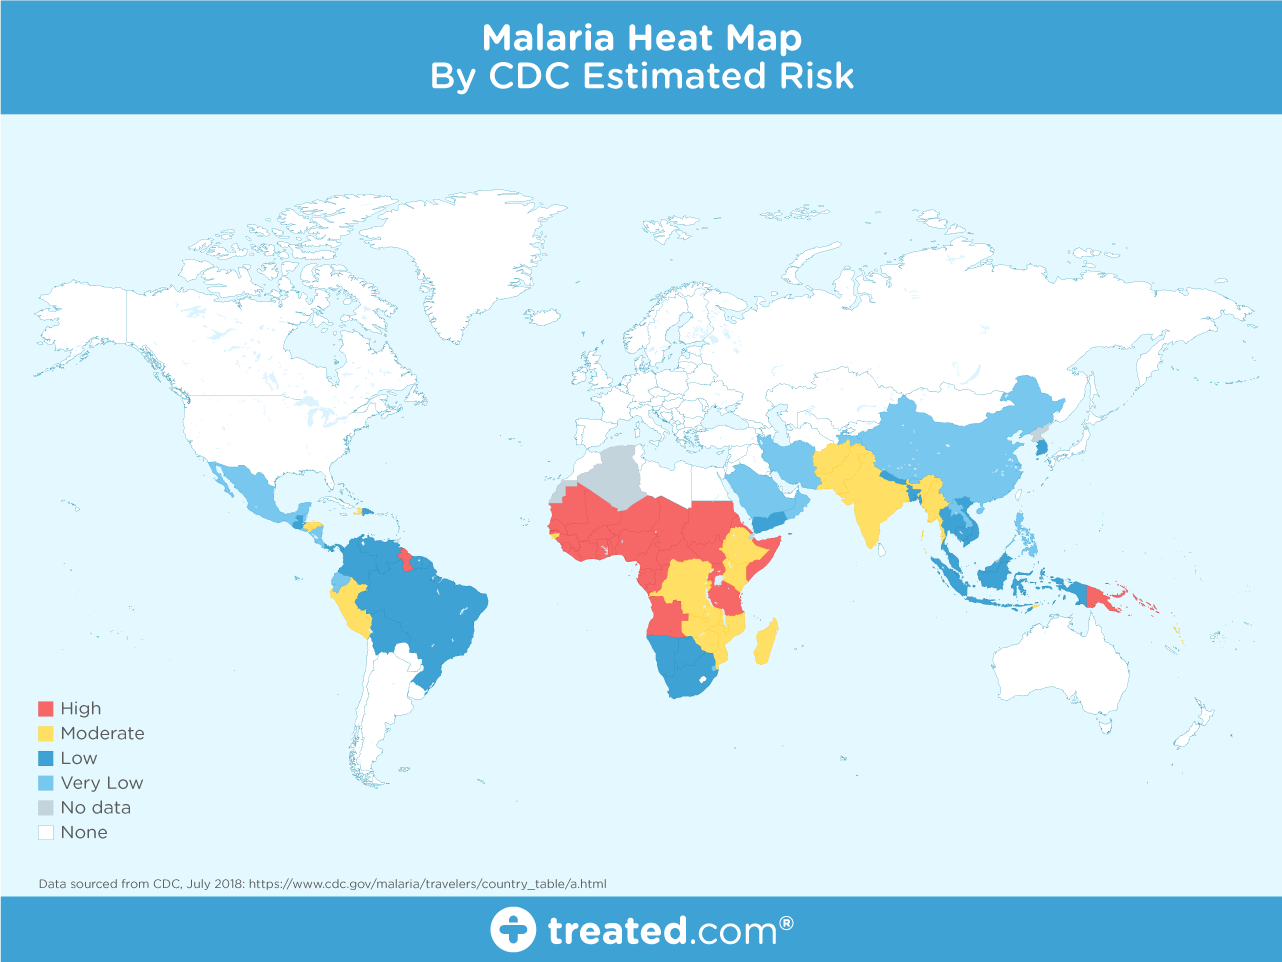
\includegraphics[scale=0.18]{img/malaria_heatmap}
\end{frame}


\begin{frame}[fragile]
  \frametitle{Malaria Diagnosis}
  Microscopic examination of blood is the best known method for diagnosis of malaria. A patient’s blood is smeared on a glass slide and stained with a contrasting agent that facilitates identification of parasites within red blood cells. A trained clinician examines 20 microscopic fields of view at 100 X magnification, counting red blood cells that contain the parasite out of 5,000 cells.\\

  \vspace{3mm}

  \verb|https://www.youtube.com/watch?v=VgDeKRC_1qk|
\end{frame}

\begin{frame}[fragile]
  \frametitle{Malaria Diagnosis}
  With regular manual diagnosis of blood smears, it is an intensive manual process requiring proper expertise in classifying and counting the parasitized and uninfected cells. Typically this may not scale well and might cause problems if the right expertise in specific regions around the world is not available.\\

  \vspace{3mm}

  Deep Learning models have proven to be really effective in a wide area of computer vision tasks.\\

  \vspace{3mm}

  Let's try to diagnose Malaria with a deep learning model!
  \end{frame}
